\documentclass[12pt,a4paper]{article}
\usepackage{graphicx}
\usepackage{caption}
\usepackage{subcaption}
\usepackage{chemformula}
\usepackage[margin=0.75in]{geometry}
\usepackage[colorlinks=true,linkcolor=blue,urlcolor=black,bookmarksopen=true]{hyperref}
\usepackage{bookmark}
\usepackage[utf8]{vietnam}
\title{Ảnh hưởng của chiếu xạ gamma lên các thuộc tính của cao su tái chế/ cao su hỗn hợp nitrile - butadiene và sự trương phình của nó trong động cơ và dầu hãm.}
\author{
Medhat M Hassan, Raouf O Aly , AH El-Ghandour and Heba A Abdelnaby}
\date{\today}
\begin{document}\maketitle
	\tableofcontents
	\newpage
	\section{Đặt vấn đề}
	
Bột cao su tái chế (Reclaimed rubber powder - RRP) trộn kèm glycidyl methacrylate (GMA) nhằm đạt được những tính chất phù hợp nhằm tăng khả năng chịu dầu. Hỗn hợp GMA-RRP (Glycidyl methacrylate - Reclaimed rubber powder) được sản xuất bằng cách trộn với cao su nitrile-butadien (NBR) trong hỗn hợp nhiều thành phần. Sau đó, hỗn hợp được chiếu xạ với liều 50 đến 200 kGy. Các thuộc tính của hợp chất sau pha trộn được đánh giá kỹ lưỡng bằng cách sử dụng phương pháp quang phổ chuyển đổi hồng ngoại Fourier (Fourier transform infrared spectroscopy) và kính hiển vi điện tử quét (scanning electron microscopy - SEM). Các thuộc tính khác nhau của chế phẩm tổng hợp không qua chiếu xạ và hỗn hợp được chiếu xạ như là độ kéo căng , độ giãn nở tối đa, độ cứng, khả năng trương phình của vỏ lốp ô tô và khả năng chịu dầu và tính ổn định nhiệt được khảo sát mối liên quan của các thành phần trong bột cao su tái chế ( RRP). Kết quả cho thấy rằng độ kéo căng, độ cứng và khả năng hạn chế trương phình (swelling resistance) được tăng cường khi tăng hàm lượng cao su nitrile-butadien (NBR) trong hỗn hợp. Cụ thể, độ kéo căng tăng lên theo liếu chiếu có giá trị trong khoảng từ 50 - 200 kGy. Tỷ lệ phần trăm khối lượng còn dư của hỗn hợp tăng lên rõ rệt khi kết hợp với RRP gia tăng. Tỷ lệ phần trăm trương phình giảm đều đặn khi tăng liều bức xạ gia tăng, điều này do sự khâu mạch được hình thành bới bức xạ .\\

\textbf{Từ khoá}: NBR, bột cao su tái chế (reclaim rubber), bức xạ gamma (gamma radiation), tính cơ học (mechanical), tính bề nhiệt (thermal), độ trương phình (swelling), thuộc tính hình thái (morphological properties)

	\section{Phần giới thiệu}
\vspace{0.4em}
Cao su acrylonitrile-butadiene (NBR) được thương mại hóa trong hơn 50 năm. NBR được biết đến với giá rẻ , khả năng chịu dầu tuyệt vời, dầu mỡ, tính thấm thấm thấp và quá trình thực hiện dễ dàng. NBR tự chuyển đổi thành loại cao su nối mạch do các liên kết chéo (cross-linking rubber) khi chiếu bức xạ năng lượng cao. Điều đáng chú ý là khi phơi chiếu các loại polyme hình thành liên kết chéo với bức xạ, làm tăng tính ổn định và tính chất cơ học. Tuy nhiên, liều bức xạ cao phải phù hợp để đạt được mật độ liên kết chéo mong muốn. Tuy nhiên, ở mức liều bức xạ cao hơn, các tính chất cơ học bị tác động nghiêm trọng do sự thoái hoá gây ra bởi bức xạ. Việc áp dụng nó trong công nghiệp chế tạo lốp ô tô rất đa dạng, nhưng khả năng chống lão hóa bị hạn chế do mạch chưa bão hòa butadiene. Cấu trúc của mạch NBR được thể hiện dưới đây:
   

	\begin{figure}[h]
		\centering
		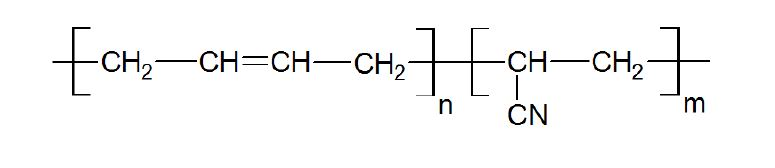
\includegraphics[width=0.4\textwidth]{1.jpg}
		\caption{Cấu trúc mạch NBR}
		\vspace{0.4em}
	\end{figure}
	
Với lượng phế thải polymer ngày càng tăng là một vấn đề nghiêm trọng đáng chú ý. Trong số chất thải polymer này, chỉ có 8-12\% là nhựa, trong khi đa phần là chất thải đàn hồi (elastomer). Điều khó khăn trong việc tái chế lốp xe bởi vì vỏ lốp xe phế thải là một chất kết dính chéo nên rất khó nấu chảy và xử lý. Có nhiều loại quy trình tái chế bằng phương pháp vật lý được áp dụng như là các phương pháp cơ học, cơ nhiệt, sóng cực ngắn và siêu âm. Cao su tái chế từ cao su phế phẩm, được áp dụng như một chất thay thế tối ưu cho cao su nguyên chất trong vô số loại cao su tổng hợp. Điều này mở ra hướng đi mới cho lộ trình tái chế cao su phế phẩm, tạo ra những sản phẩm tốt với giá cả thấp hơn. Trong toàn bộ các lốp xe tái chế được lấy từ cao su phế phẩm, dạng phổ biến, một là cao su không phân cực (nonpolar rubber) như cao su tự nhiên (Natural rubber - NR), cao su styrene-butadiene (SBR) và cao su butadiene (BR) và hai là cao su phân cực (polar rubber) như là cao su Acrylonitrile–butadiene (NBR) cũng như nhựa chịu nhiệt (thermoplastic).\\

Sự ảnh hưởng của bức xạ ion hoá lên hỗn hợp polyme tái chế từ cao su phế thải (Waste rubber - WR) đã được nghiên cứu rõ ràng. Một số thí nghiệm được tiến hành nhằm đánh giá khả năng kết hợp bột cao su phế thải (ground rubber powder - GRP) và cao su loại bỏ lưu hoá (devulcanized rubber waste) làm chất độn và một phần của cao su tự nhiên (NR - nature rubber). Cao su mới được tạo ra từ bột cao su phế thải - GRP và cao su loại bỏ lưu hoá lấy từ lốp xe chở khách và xe tải nhỏ, có nhiều đặc tính cơ học hữu ích, và tính cơ học tốt hơn nhiều so với cao su phế thải – GRP đơn thuần. Nghiên cứu gần đây được thực hiện khi sử dụng GTR để sản xuất nhựa chịu nhiệt bao gồm PE, cao su tinh khiết và GTR có và không có chất oxy hóa.\\

Mục đích của nghiên cứu này là nghiên cứu đánh giá sự sự ảnh hưởng của chiếu xạ gamma qua các tiêu chí về tính cơ học, tình chịu nhiệt và khả năng trương phình trong dầu động cơ và dầu hãm. Nhằm làm sáng tỏ các yếu tố kết hợp trong pha trộn được đánh giá bằng phương quang phổ hồng ngoại chuyển đổi (Fourier transform infrared spectroscopy - FTIR) và kính hiển vi điện tử quét (SEM). Các tính chất của hỗn hợp đã được nghiên cứu và đánh giá trước và sau khi chiếu xạ. Sản phẩm được phát triển là hướng đi mới trong việc áp dụng rộng rãi trong ngành công nghiệp ô tô và ứng dụng con dấu và gioăng.\\
	\section{Phần chuẩn bị thí nghiệm}%% PHAN 3
		\subsection{Chuẩn bị vật liệu}
		Bột cao su tái chế (RRP) với kích thước hạt là 80 mesh (150 mm) từ cao su phế thải (GR) trong mặt lăn lốp xe, cạnh sườn lốp xe của xe khách và xe tải được cung cấp bởi công ty Narobine, Cairo, Ai Cập. NBR, dưới tên thương mại lài KRYNAC 4050 được cung cấp bởi công ty Bayer, Đức, có hàm lượng acrylonitrile trung bình là 30 wt\%. Độ nhớt Mooney ML1 + 4 (1000C) 50 + 5 and mật độ 0.98 g/cm3. Tác nhân phản ứng glycidyl methacrylate (GMA) được cung cấp bởi công ty Merck, Đức. Hình \ref{fig:hinh2} – Tác nhân phản ứng - glycidyl methacrylate (GMA)
		\begin{figure}
			\centering
			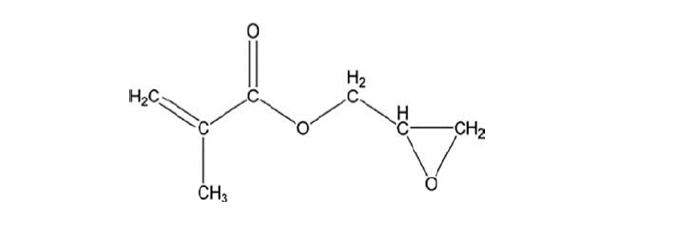
\includegraphics[width=0.8\textwidth]{2.JPG}
			\caption{Tác nhân phản ứng (GMA)}	
			\label{fig:hinh2}	
		\end{figure}
		
		\subsection{Chuẩn bị bảng tấm cao su}
		Các hỗn hợp RRP / NBR / GMA trộn với nhiều thành phần khác nhau được chuẩn bị để đem vào thiết bị nghiền trộn hoạt động như máy nghiền Brabender. Sau khi đun nóng NBR, thêm bột cao su tái chế RRP vào máy, trộn trong khoảng 10 phút ở nhiệt độ $170 - 175 ^o C$ để đồng nhất RRP vào NBR. Sau đó thêm tác nhân phản ứng GMA 2 wt\% vào hỗn hợp này. Sau khi trộn, các mẫu được ép nóng ở nhiệt độ $175^o C$, áp suất 10 MPa trong 5 phút trong các bảng ép (Sheet) để có độ dày và kích thước phù hợp cho phân tích.
		\subsection{Chiếu xạ gamma}%%OK
		Các hỗn hợp sau khi trộn được chiếu xạ gamma (tế bào gamma (cell gamma) loại 4000 A, xuất xứ Ấn Độ), trong không khí, ở nhiệt độ phòng và ở độ ẩm môi trường xung quanh. Liều hấp thụ là 50, 100, 150, 200 và 250 kGy ở suất liều chiếu 5 kGy / h. Viêc chiếu xạ được thực hiện tại Trung tâm Quốc gia về Nghiên cứu và Công nghệ bức xạ, Cơ quan Năng lượng nguyên tử, Cairo, Ai Cập.
		\subsection{Tiến hành đo độ bền cơ học}%% ok
		Kiểm tra độ kéo căng của các mẫu hợp chất sau khi trộn được xác định bằng hệ thống máy Hounsfield , Anh. Các đánh giá về độ kéo giãn, độ giãn nỡ tối đa (elongation at break) dựa trên thông số tương ứng của Tổ chức tiêu chuẩn đo lường Quốc tế (ISO) 37-1977 (E) và ISO 34-1975 (E) .
		\subsection{Đo độ cứng}%% OK
		Các mẫu có độ dày ít nhất 1mm được cắt ra để kiểm tra độ cứng. Kiểm tra đo lường được tiến hành tại Hiệp hội Kiểm định và Vật liệu Mỹ (ASTM) D 2240 (American Society for Testing and Materials - ASTM) D 2240 (ASTM, 2000) sử dụng máy đo Adurometer Model 306L. Đơn vị độ cứng được thể hiện trong bờ A (A Shore).
		\subsection{Phân tích độ bền nhiệt}%ok
		Phân tích nhiệt trọng (Thermogravimetric analysis - TGA) được thực hiện với hệ thống Shimadzu TGA-50 (Kyoto, Nhật Bản) và được nung ở nhiệt độ $20-600 ^oC$ với tốc độ 20 $^oC$ / phút, dưới lưu lượng khí nitơ khô là 20ml / phút. $T_{0.25}$, $T_{0.50}$ và $T_{0.75}$ là nhiệt độ Celsius mà phần trăm khối lượng mất mát 25\%, 50\% và 75\% tương ứng.
		\subsection{Đặc tính hình thái}%ok
		ISM-5400 kính hiển vi điện tử quét (JEOL, Nhật Bản) được dùng để quan sát hình dạng và nếp đứt gãy của mẫu trong nitogen lỏng được bọc vàng trước khi tiến hành thí nghiệm.
		\subsection{Phân tích phổ hồng ngoại}%Ok
		Phân tích phổ hồng ngoại được thực hiện với máy quang phổ FTIR spectrophotmeter, Mattson 100 Unican, England, với phạm vi từ 500 -  4000  $cm^{-1}$. Mẫu hỗn hợp được nghiền với 3 mmg KBr, sau đó được nén tạo dạng đĩa trong. Các mẫu phân tích hồng ngoại, trước tiên được làm khô trong chân không ở nhiệt độ 800 $^oC$ trong 2 h.
		\subsection{Kiểm tra độ trương phình}
		Độ trương phình trung bình được đo bằng phương pháp sau. Chuẩn bị 3 mẫu đồng dạng và trọng lượng ($\approx$
0.5 g) mỗi mẫu được cân chính xác (W) và ngâm trong 50 ml dung môi ở nhiệt độ phòng trong 24 giờ. Sau đó, lấy
mẫu ra ngoài và đặt giữa hai miếng giấy lọc, tất cả được đặt giữa hai tấm kính (mỗi chiếc có trọng lượng là 98,4 g)
nhằm hạn chế tác động bên ngoài trong 5 giây, cuối cùng thực hiện cân lại trong bình cân ($W_t$). Tỉ lệ phần trăm độ
trưng phình (the swelling percentage) của mỗi mẫu được tính theo công thức dưới đây: 
	\begin{eqnarray}
		Q\% = \frac{W_t - W}{W}\times 100 \%
	\end{eqnarray}
	Trong đó, W và $W_t$ lần lượt là khối lượng trước và sau khi trương phình trong khoảng thời gian ngâm (t).
Khối lượng mẫu được cân bằng cân điện tử với độ chính xác 1 mg.
	
	\section{Kết quả thí nghiệm và đánh giá}
	
	\subsection{Các thuộc tính cơ học}
	
	\begin{figure}
		\centering
		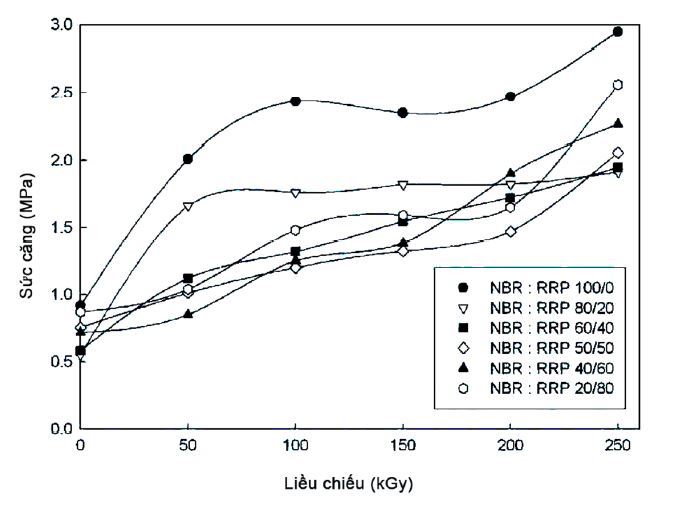
\includegraphics[width=0.9\textwidth]{3.JPG}
		\caption{Độ kéo căng của cao su nitrile–butadiene rubber (NBR) được trộn với cao su tái chế (Reclaimed
rubber powder - RRP) dùng 2\% glycidyl methacrylate (GMA) với tỉ lệ khác nhau theo liều chiếu gamma tương ứng.}
		\label{fig:HINH1}		
	\end{figure}
	
	
	Sự khác biệt của độ kéo căng (Tensile strength – Ts) với tỷ lệ trộn RRP trong NBR có GMA được thể hiện
trong Hình \ref{fig:HINH1}. Sự giảm rõ rệt độ kéo căng khi bổ sung RRP là do khối lượng phân tử trong cao su tái chế thấp hơn.
Quá trình làm biến dạng và nhiệt độ cao trong quá trình tái tạo (reclamation process) đã phá vỡ các mạch phân tử thành các đoạn ngắn hơn. Sự kết hợp của các mẫu phân tử có khối lượng nhỏ là kết quả của quá trình không ngừng nhằm giảm độ kéo căng. Ảnh hưởng của bức xạ năng lượng cao lên polymer là tạo ra các gốc tự do, kết quả của quá trình bẻ gãy các liên kết yếu. Những gốc tự do mới được hình thành này sẽ tiếp tục phản ứng với chính gốc tự do khác hoặc với oxy trong phân tử. Sự ảnh hưởng của chiếu xạ gamma với các liều chiếu khác nhau đến Ts của cao su hỗn hợp RRP/NBR/GMA nhiều thành phần được thể hiện trong hình \ref{fig:HINH1}. Độ kéo căng của mẫu tăng lên theo sự gia tăng liều chiếu xạ. Cường độ kéo căng của cao su hỗn hợp RRP/NBR/BMA tăng liên tục với liều chiếu xạ trích dẫn trong phạm vi nghiên cứu này. Điều này là do mật độ liên kết chéo trong cao su hỗn hợp hình thành bởi tác động của bức xạ năng lượng cao. Mật độ các liên kết chéo thể hiện rằng nhiều liên kết C-C trong mạng và nhiều năng lượng ngăn cản sự kéo căng.\\

	\begin{figure}
		\centering
		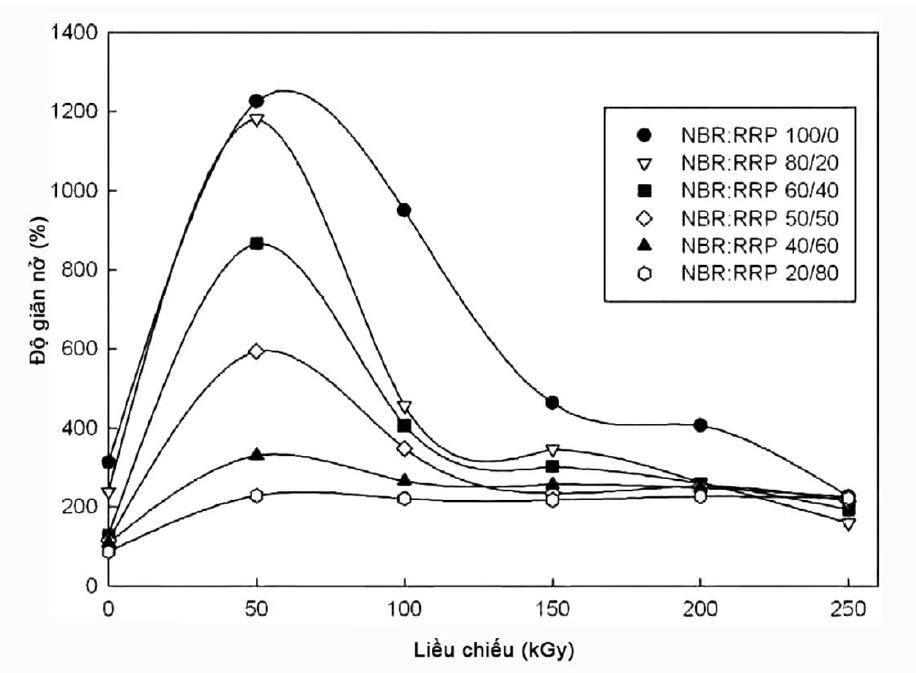
\includegraphics[width=0.9\textwidth]{4.JPG}
		\caption{Độ co giãn tối đa của cao su hỗn hợp nitrile–butadiene rubber (NBR) với tỉ lệ trộn bột cao su tái chế dùng 2\% glycidyl methacrylate (GMA) theo liếu chiếu gamma khác nhau}
		\label{fig:HINH2}		
	\end{figure}
	
	Hình \ref{fig:HINH2} thể hiện sự khác biệt của phần trăm độ giãn nỡ tối đa (Eb) của cao su hỗn hợp theo tỉ lệ trộn RRP. Giá trị Eb giảm tuần tự theo tăng tỉ lệ trộn RRP tại liều chiếu 50 kGy, có giá trị giảm chậm từ 1225 xuống 228\% tương ứng với sự tăng tỉ lệ trộn RRP từ 0 đến 80\%. Trong phân tử khối lượng nhỏ và hiện diện của chất độn trong RRP tinh khiết có thể kiềm chế các phân tử định hướng đó là nguyên nhân làm độ co giãn của mẫu thấp. Cũng thế, ghi nhận được rằng sự hiện diện của liên kết chéo trong hạt cao su và các hạt thành phần trong bột cao su RRP, nó mất khả năng co giãn khi biến dạng, vì thế giới hạn khả năng linh động của hỗn hợp, đặc biệt ở cao su có hàm lượng cao RRP. \\
	
	
	Từ hình \ref{fig:HINH2}, khi tăng liều chiếu, trong toàn bộ hỗn hợp với Eb tăng dần đều đến liều 50 kGy và sau đó giảm dần. Điều này thể hiện, các liên kết chéo được hình thành trong hỗn hợp với liều chiếu xung quanh 50 kGy và ở liều chiếu thấp thì hình thành các liên kết không bắt chéo trong hỗn hợp hoạt động như chất nhựa dẻo, vì thế giá trị Eb tăng, trong khi hỗn hợp pha trộn thì giá trị Eb giảm với sự tăng liều chiếu. Sự suy giảm này là do sự hình thành các liên kết chéo trong cấu trúc vật liệu. Tuy nhiên, với mật độ liên kết chéo cao, mạng cấu trúc trở nên dày đặc, do đó có ít năng lượng hao phí trong mạng và cần nhiều năng lượng để phá vỡ liên kết. Ở tại các mạng có mật độ liên kết chéo cao, các đại phân tử trở nên thụ động, dó đó mạng trở nên cứng chắc hơn và tính đàn hồi giảm.
	
	\begin{figure}
		\centering
		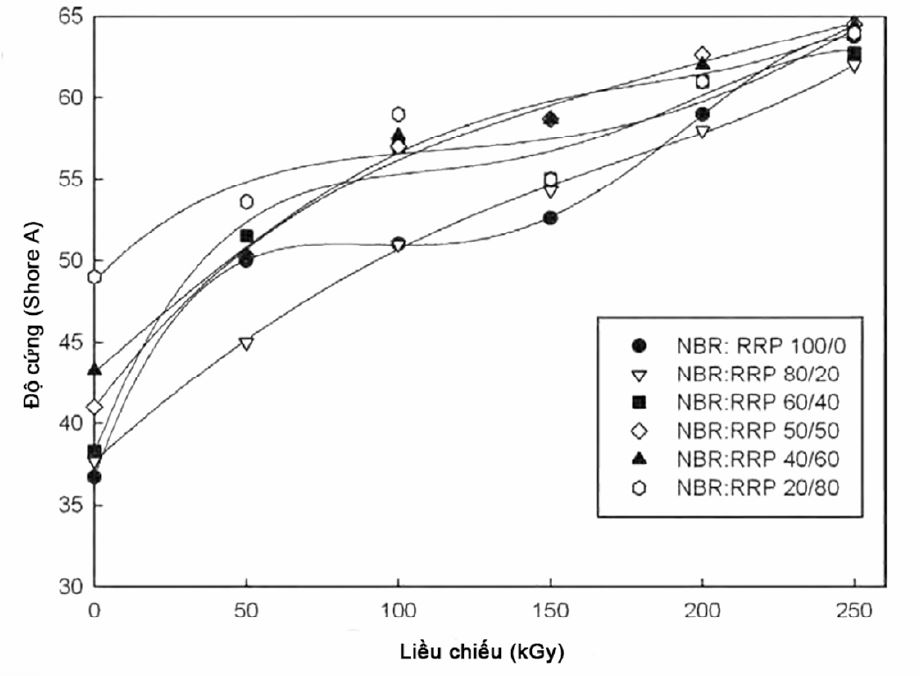
\includegraphics[width=0.9\textwidth]{5.JPG}
		\caption{Thể hiện sự thay đổi độ cứng của cao su nitril-butadien (NBR) trộn với bột cao su tái chế (RRP) với các tỷ lệ khác nhau có 2\% glycidyl methacrylate (GMA) theo liều chiếu gamma khác nhau}
		\label{fig:HINH3}		
	\end{figure}	
	
	Sự khác biệt về độ cứng của cao su NBR tinh khiết và cao su hỗn hợp RRP / NBR / GMA với nhiều thành phần được chiếu xạ gamma với liều khác nhau được minh họa trong Hình \ref{fig:HINH3}. Dữ liệu về cao su không được chiếu xạ được đưa vào cùng để so sánh với mẫu. Có thể nhận thấy rằng giá trị về độ cứng tăng lên hiệu quả bằng cách tăng mức độ pha trộn RRP. Các tính chất đạt được của cao su hỗn hợp được chiếu xạ khi so sánh về độ cứng ở cùng liều chiếu. Mặt khác, sự gia tăng tương đối đạt được với giá trị độ cứng mẫu cao su giống nhau về thành phần tăng theo liếu chiếu từ 50 – 250 kGy. Các dữ liệu trên rõ ràng cho thấy độ cứng tăng lên là sự đóng góp của các liên kết chéo hình thành do bức xạ trong mạng cao su vô định hình của mẫu là đáng kể.
	
	
	
	
	\subsection{Độ ổn định nhiệt của Polymer tinh khiết và cao su hỗn hợp qua xử lý}
Bảng 1. Dự liệu kết quả đo TGA của hỗn hợp không chiếu xạ và chiếu xạ của cao su tái chế RRP / NBR với liều chiếu tương ứng 100 và 200 kGy\\
	\begin{figure}[h]
			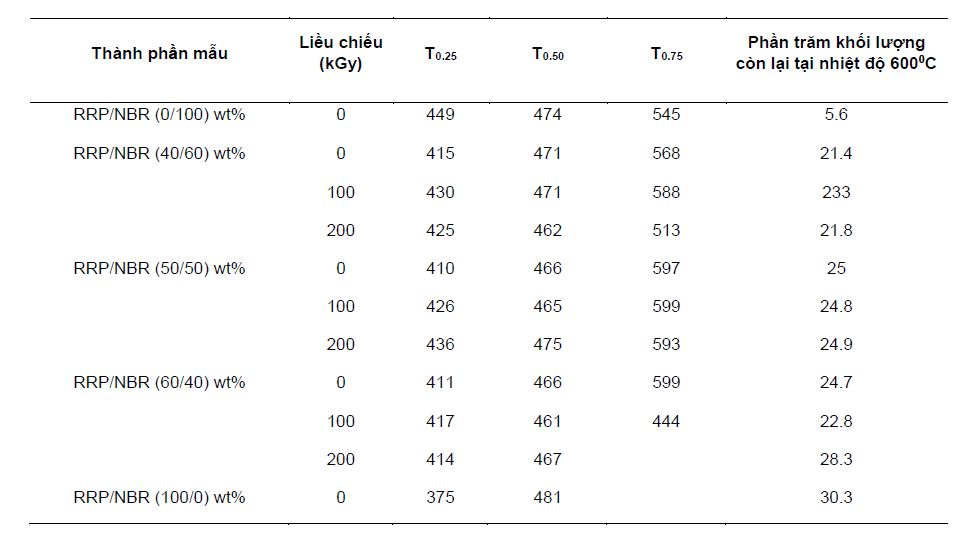
\includegraphics[width=0.9\textwidth]{BANG1.JPG}		
			\label{fig:BANG1}
	\end{figure}
	
	Phân tích nhiệt độ thoái biến của cao su NBR, RRP và RRP / NBR / GMA bằng phương pháp nhiệt trọng được xem là một trong những kỹ thuật được áp dụng rộng rãi để đánh giá sự ổn định nhiệt của các polymer trong phạm vi nhiệt độ rộng. Kết quả đo ban đầu của phương pháp TGA cho cao su NBR không bị chiếu xạ và chiếu xạ với cao su NBR trộn kèm cao su tái chế RRP được thể hiện trong Hình \ref{fig:HINH4} và hình 7. Đồng thời, bảng 1 tóm tắt sự hao hụt khối lượng ở nhiệt độ 600$^oC$ tại đó sự mất mát khối lượng khác nhau với các tỷ lệ trộn thành phần RRP khác nhau trước và sau khi chiếu xạ gamma.\\
	
	\begin{figure}
		\centering
			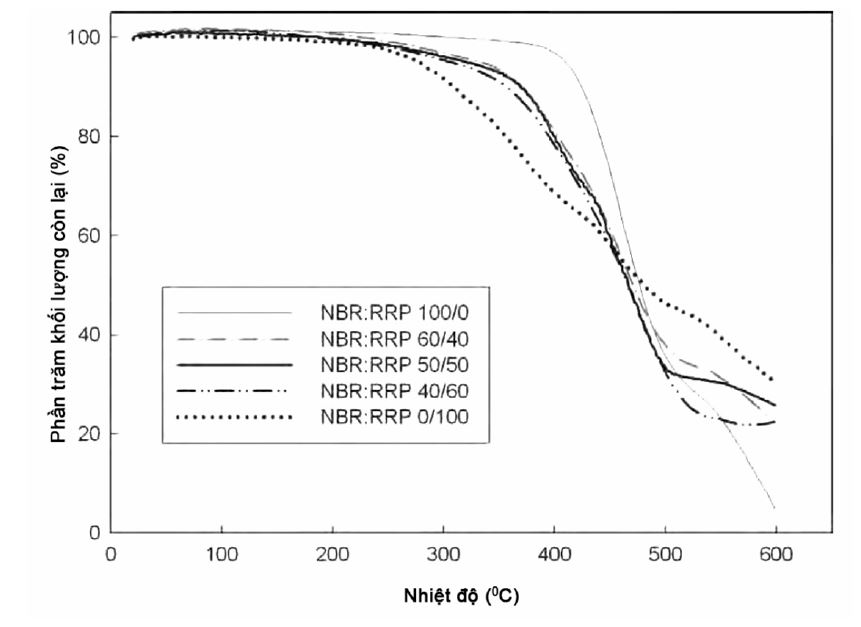
\includegraphics[width=0.9\textwidth]{6.JPG}
			\caption{Thể hiện phân tích nhiệt trọng (Thermogravimetric analysis - TGA) đối mẫu NBR không chiếu xạ với tỉ lệ trộn RRP dùng 2\% GMA}
			\label{fig:HINH4}
	\end{figure}
	
Như có thể thấy từ hình \ref{fig:HINH4}, sự bắt đầu của quá trình thoái biến tại $T_{0.25}$ là 449 $^oC$, trong khi $T_{0.50}$ là 474 $^0C$ và $T_{0.75}$ là ở 545 $^0C$. Do đó, mẫu RRP / NBR / GMA (0/100/2 wt\%) được đánh giá là ổn định nhiệt có lên đến 449 $^0C$. Ở trên 449 $^0C$, quá trình nóng chảy bay hơi diễn ra nhanh chóng và hầu như mẫu hoàn toàn bị phân hủy. Do đó, không có sự mất mát khối lượng đáng kể trong nhiệt biểu trên nhiệt độ này được phát hiện. Sự ảnh hưởng của tỷ lệ pha trộn hỗn hợp được ghi nhận trên TGA được trình bày trong cùng một hình. So sánh với mô hình suy thoái của từng thành phần, hoạt tính suy giảm của hỗn hợp là khác nhau (Bảng 1).\\

\begin{figure}
	\centering
	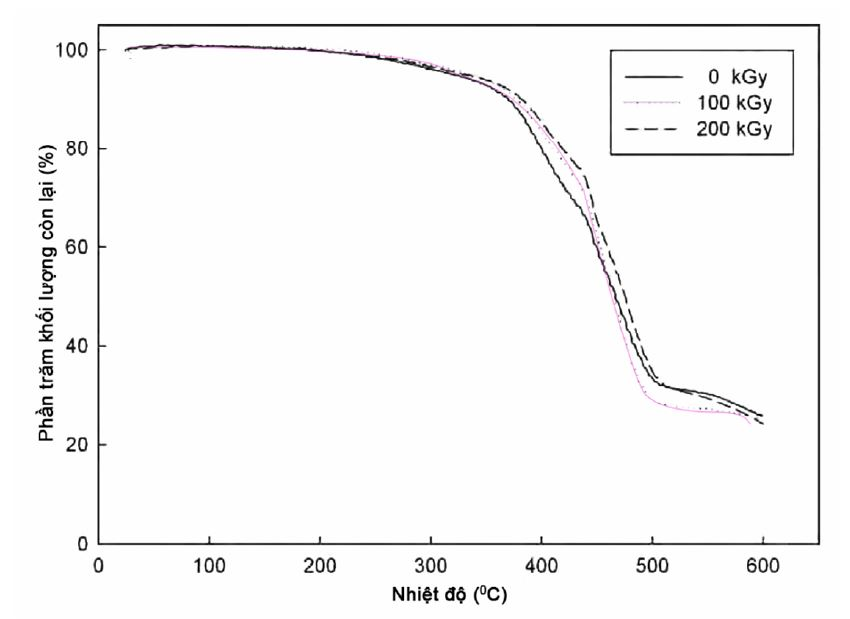
\includegraphics[width=0.9\textwidth]{7.JPG}
	\label{fig:HINH5}
			\caption{Thể hiện kết quả phân tích nhiệt trọng (TGA) của cao su hỗn hợp NBR/RRP/GMA (50/50/2 wt\%) theo liều chiếu xạ tương ứng.}
\end{figure}
		
	Như được trình bày trong Bảng 1, nhiệt độ thoái biến giảm dần bằng cách thêm vào bột cao su phế thải (Waste rubber – WR) trong hỗn hợp. Bảng 1, thể cũng cho tỷ lệ phần trăm mất mát khối lượng trong mẫu ở ba nhiệt độ khác nhau, $T_{0.25}$, $T_{0.5}$ và $T_{0.75}$. Khi phần trăm khối lượng của cao su phế thải WR trong hỗn hợp này tăng lên, một nhận thấy rằng sự giảm dần dần độ mất mát khối lượng, gia tăng độ ổn định nhiệt. Nhiệt biểu TGA ban đầu và tỷ lệ đường phản ứng đối với các hỗn hợp chiếu xạ có chứa RRP / NBR / GMA, (50/50/2 wt\%) được thể hiện trong hình \ref{fig:HINH5}. Như đã thấy trong Bảng 1, sự ổn định nhiệt độ tối ưu đã đạt được với cao su hỗn hợp RRP / NBR / GMA, tỉ lệ trộn (40/ 60/2 wt\%), nhờ đó sự ổn định nhiệt tăng lên cùng với sự gia tăng liều bức xạ, như được báo cáo cho hỗn hợp 50/50, điều này cho thấy rằng các liên kết chéo giữa phân tử được hình thành khi chiếu bức xạ. Tỷ lệ phần trăm khối lượng còn lại trong hỗn hợp rõ ràng tăng lên khi gia tăng hàm lượng RRP.\\
	
	\subsection{Phân tích FTIR}
	
		\begin{figure}
			\centering
			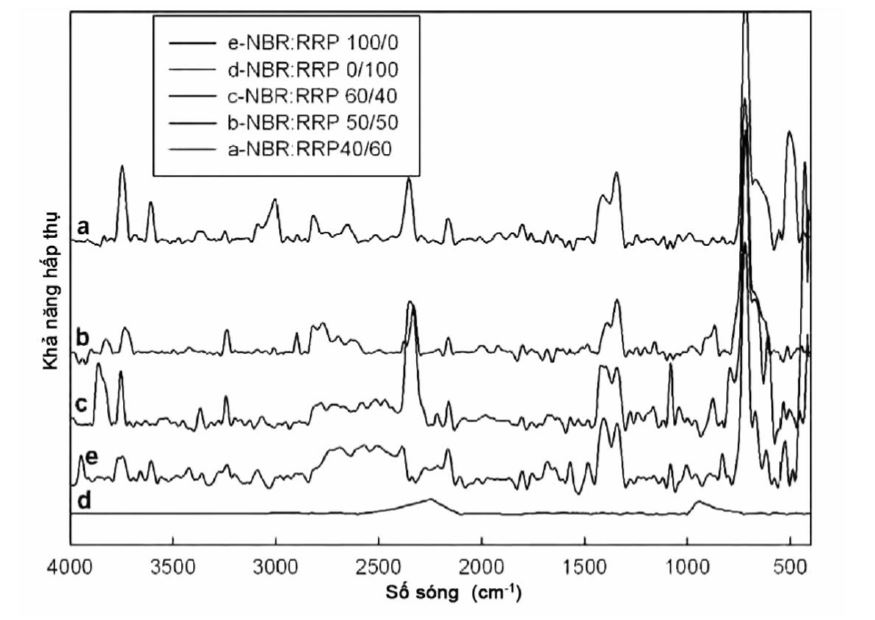
\includegraphics[width=0.9\textwidth]{8.JPG}
			\label{fig:HINH_6}
			\caption{Đồ thị thể hiện độ trương phình theo thời gian của NBR với RRP thay thế từng phần cho NBR/RRP/GMA trong dầu động cơ.}
		\end{figure}
			
	Nghiên cứu sự thay đổi tính chất hoá học của mạng polymer khi chiếu xạ bằng phương pháp quang phổ hồng ngoại chuyển đổi (FTIR). Hình \ref{fig:HINH_6}, thể hiện Phổ FTIR trong phạm vi 400 – 400 $cm^{-1}$ của bột cao su RRP, cao su NBR và cao su hỗn hợp của chúng có GMA so với cao su trong lốp xe. Tại 1090 $cm^{-1}$ trong phổ được chỉ định là carbon để đối chiếu tham khảo. Dùng lại phổ phân tích cao su lốp xe ở dãi thấp tại 1723 $cm^{-1}$, thấy được mối liên hệ với sự oxy hoá nhiệt (thermal oxidation) là kết quả của quá trình tiếp xúc bề mặt với oxy và gây ra sự hình thành lớp oxy hoá gồm có các nhóm carbonyl. Dải mạnh tại 1587 $cm^{-1}$ thì liên quan đến liên kết C=C trong polyisoprene, dải mạnh ở 2336 $cm^{-1}$ thì được cho là liên kết \ch{{C+N} -} trong mạch, trong dải tại 1412 $cm^{-1}$ thì được nhận định là \ch{=CH2} dao động kiểu cây kéo, dải phổ tại 839 $cm^{-1}$ là monome \ch{[-C(CH3)=CH-]} và dải phổ tại 479 $cm^{-1}$ liên quan đến liên kết \ch{S-S}. Phổ của cao su NBR được vẽ trên cùng một hình, và độ bão hoà của methy/methylene dao động trong 2800-3000 $cm^{-1}$, và nitrile dao động trong khoảng 2240 $cm^{-1}$ thì được quan sát. Một số bài viết chỉ ra rằng không có thay đổi đã được quan sát trong dải bất định CN. Đỉnh nhỏ tại 2183 $cm^{-1}$, có thể do sự liên hợp của nhóm nitrile không thay đổi trong suốt quá trình chiếu xạ.\\
	
	\begin{figure}
			\centering
			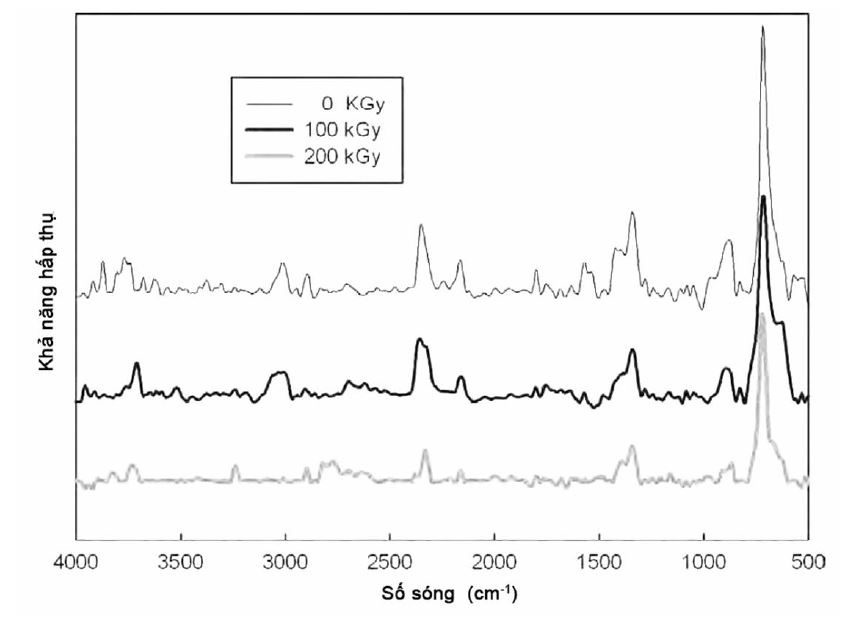
\includegraphics[width=0.9\textwidth]{9.JPG}
			\label{fig:HINH_7}
			\caption{Đồ thị thể hiện độ trương phình theo thời gian của NBR với RRP thay thế từng phần cho NBR/RRP/GMA trong dầu động cơ.}
		\end{figure}
	
	
	Hình \ref{fig:HINH_7}, thể hiện phổ FTIR của mẫu cao su RRP không chiếu xạ và cao su hỗn hợp của nó với NBR với tỉ lệ trộn khác nhau. Các hợp chất hydrocarbon được mô tả bởi dải mạnh với nhiều đỉnh gần 2813 $cm^{-1}$ và khoảng giữa 1451 và 1334 $cm^{-1}$. Các dải tương ứng với nhiều dạng dao động giãn khác nhau của chuỗi \ch{–CH2}. Đặc trưng của dải phổ tương ứng với dao động co giãn của \ch{–C-H} của nhóm \ch{CH3}, xấp xỉ tại 1370 $cm^{-1}$ có thể nhìn thấy. Ngoài ra, dải phổ mạnh với nhiều đỉnh có cường độ trung bình trong phạm vi 1250-883 $cm^{-1}$. Trong dải phổ của NBR, tại 2350 $cm^{-1}$ thì được quy ra dao động kiểu kéo giãn của alkyl \ch{–C-N}, cường độ dao động tăng lên với hàm lượng NBR, trong khi dải phổ tại 960 $cm^{-1}$ là do dao động kiểu vẫy tay của butadiene. Đặc trưng của dải hấp thụ của hỗn hợp polymer là dao động kiểu co kéo giãn của \ch{-{C-O} -} tại 1672 $cm^{-1}$, dao động kiểu biến dạng của \ch{N-H} tại 1539 $cm^{-1}$, dao động kiểu co giãn của \ch{–C+N} tại 1270 $cm^{-1}$ và dao động kiểu uốn cong của \ch{–C-O} và \ch{–N-H} trong phạm vi 580 – 690 $cm^{-1}$.\\
	
	
	Chỉ có những thay đổi thứ yếu được gây ra bởi chiếu xạ (thể hiện trong hình \ref{fig:HINH_7}). Người ta cho rằng trong cao su NBR, liên kết đôi góp phần tăng hiệu quả các liên kết chéo, nguyên nhân là do phản ứng của gốc tự do với những liên kết đôi. Mức độ liên kết chéo hình thành bởi bức xạ có thể đánh giá trực tiếp thông qua cường độ ánh sáng hồng ngoại (IR intensity) tại 1655 $cm^{-1}$ (\ch{C=C}) và tại 965 $cm^{-1}$ (transvinylidene \ch{C=C}) hoặc tại 1446 $cm^{-1}$ ( biến dạng methylene gây ra bởi \ch{C=O}). Một cách tổng thể, sự gia tăng mức độ hấp thụ giữa 1660 và 1750 $cm^{-1}$ chủ yếu ghi nhận và có thể là do oxy hoá (\ch{C=O}, \ch{C – O – C} ) và liên hợp của \ch{-C+N -} hoặc \ch{-C+C -}. Một đỉnh nhỏ xung quanh 3370 $cm^{-1}$, đặc biệt với liều chiếu cao, có thể là do oxy hoá hoặc sự hiện diện \ch{-C+N -H} trong mạch.\\

	\subsection{Độ chịu dầu của polymer tinh khiết và hỗn hợp qua xử lý}
	
	Độ chịu dầu là một trong những đặc điểm quan trọng để đánh giá hiệu quả sử dụng của cao su, đặc biệt là trong các ngành công nghiệp ô tô, công nghiệp chế biến cao su và ứng dụng con dấu và gioăng trong động cơ (seal applications). Độ chịu dầu thì tỉ lệ nghịch với độ trương phình là cạnh tranh động lực giữa lực tương tác về phía trước nhằm “hoà tan cao su trong dầu có khối lượng nhỏ”, (đó là khả năng trương phình) và lực đàn hồi tăng lên khi hấp thụ nhiều dầu.
		\begin{figure}
			\centering
			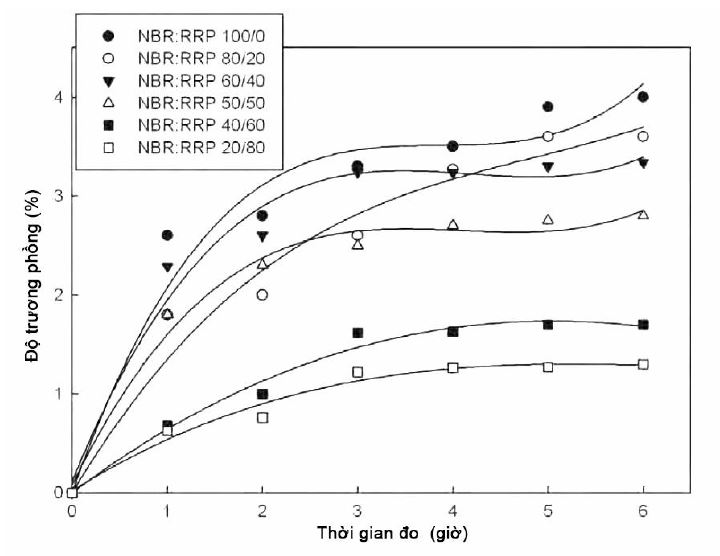
\includegraphics[width=0.9\textwidth]{10.JPG}
			\label{fig:HINH_8}
			\caption{Đồ thị thể hiện độ trương phình theo thời gian của NBR với RRP thay thế từng phần cho
NBR/RRP/GMA trong dầu động cơ}
		\end{figure}
		
		\begin{figure}
			\centering
			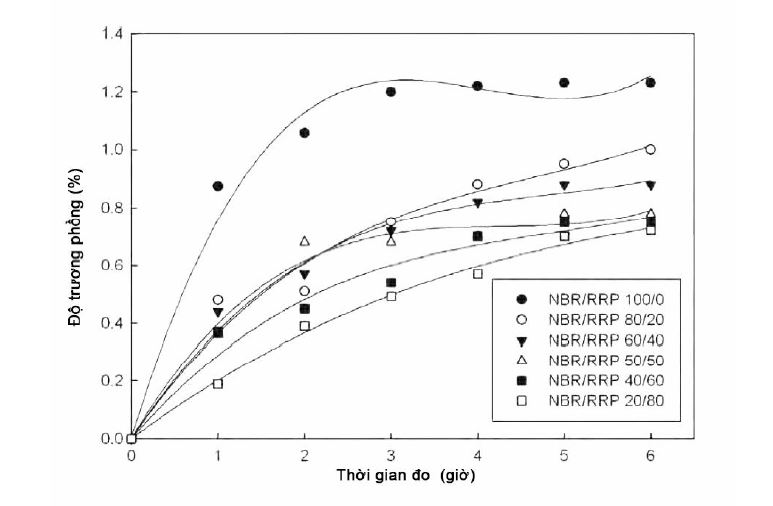
\includegraphics[width=0.9\textwidth]{11.JPG}
			\label{fig:HINH_9}
			\caption{Đồ thị thể hiện độ trương phình theo thời gian của NBR với RRP thay thế từng phần NBR/RRP/GMA trong dầu hãm.}
		\end{figure}
		
		\begin{figure}
			\centering
			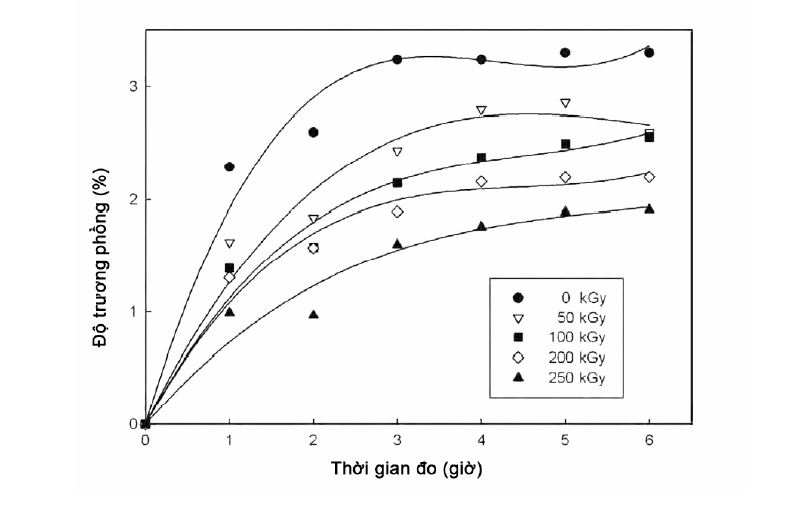
\includegraphics[width=0.9\textwidth]{12.JPG}
			\label{fig:HINH_10}
			\caption{Đồ thị thể hiện độ trương phình theo thời gian của cao su hỗn hợp NBR/RRP/GMA (50/50/2 wt\%) trong dầu động cơ được chiếu xạ gamma với liều chiếu khác nhau}
		\end{figure}
		
	Độ kháng dầu của cao su là một trong những đặc điểm quan trọng trong việc lựa chọn cuối cùng của cao su được sử dụng, đặc biệt là trong các ngành công nghiệp ô tô, và các ứng dụng con dấu. Kháng dầu là nghịch đảo của mức độ sưng trong dầu và được điều chỉnh bởi sự cạnh tranh giữa động lực hướng tới " giải thể cao su trong dầu trọng lượng phân tử thấp, " đó là sưng, và lực đàn hồi tăng khi dầu hấp thụ. 
	Hình \ref{fig:HINH_8} và \ref{fig:HINH_9} cho thấy ảnh hưởng của việc thay thế một phần NBR bằng RRP lên hành vi sưng của hỗn hợp RRP / NBR / GMA trong dầu động cơ ASTM và dầu phanh, tương ứng trong 7 ngày. Sự cân bằng sưng đã đạt được sau 6 h. Có thể lưu ý rằng tỷ lệ sưng giảm khi tăng hàm lượng RRP trong hỗn hợp. Kết quả ghi nhận sự hình thành các liên kết chéo của các hạt cao su với các thành phần khác có trong bột cao su RRP, nó có thể bị giới hạn bởi độ hoà tan dung môi của hỗn hợp đặc biệt là ở hàm lượng RRP cao hơn. Và nó được tìm thấy trong các mẫu cao su hỗn hợp mà loại dầu được lựa chọn phải tuân theo động lực học hấp thụ bậc nhất (the first-order absorption kinetics), và giá trị hằng số căng động học (the swelling kinetic constant K) tại trạng thái cân bằng đối với dầu động cơ cao hơn dầu hãm với cái tỉ lệ pha trộn khác nhau. Điều đó có nghĩa rằng độ hấp thụ dầu (oil-absorption rate) của hỗn hợp mạng trong dầu động cơ cao hơn dầu hãm. Đây là cơ sở để tin rằng độ nhớt của dầu động cơ nhỏ dầu hãm, và các phân tử của nó thì có thể khuếch tán vào trong các mạng liên kết chéo. Những kết quả thu được sau khi chiếu xạ các mẫu. Mối liên hệ của sự giảm giá trị phần trăm sức căng của các mẫu được chiếu xạ đáng chú ý khi so sánh với những mẫu không chiếu xạ tương ứng. Đó là một thực tế rằng sự gia tăng mức độ hình thành liên kết chéo là kết quả của sự hình thành một mạng dày đặc và giảm chiều dài của chuỗi giữa các liên kết và do đó giảm độ hấp thụ dầu.
.		
		
		
		
		
		\begin{figure}
			\centering
			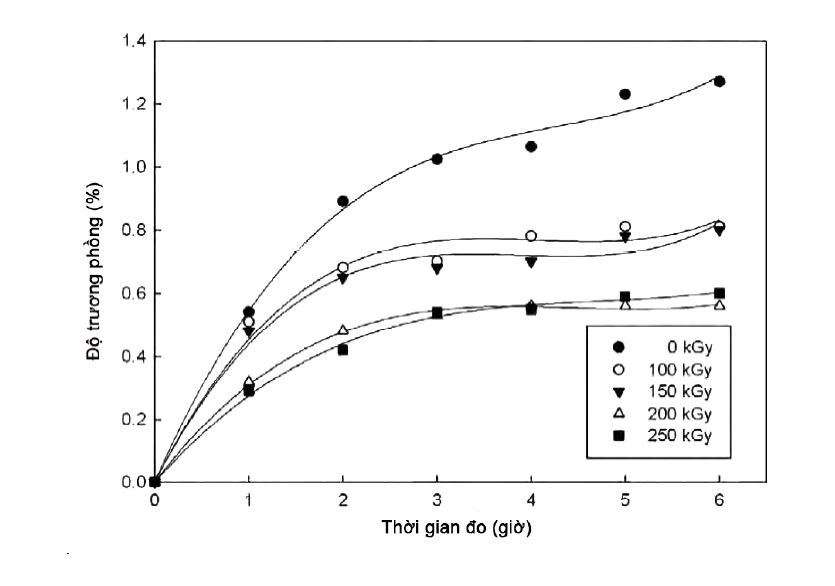
\includegraphics[width=0.9\textwidth]{13.JPG}
			\label{fig:HINH_11}
			\caption{Mối liên hệ giữa độ trương phình theo thời gian của cao su hỗn hợp NBR/RRP/GMA (50/50/2 wt\%) trong dẫu hãm ở tại những liều chiếu gamma tương ứng.}
		\end{figure}
		
	
	\subsection{Kiểm định bằng phương pháp kính hiển vi điện tử quét (SEM - scanning electron microscope)}
	
	\begin{figure}
			\centering
			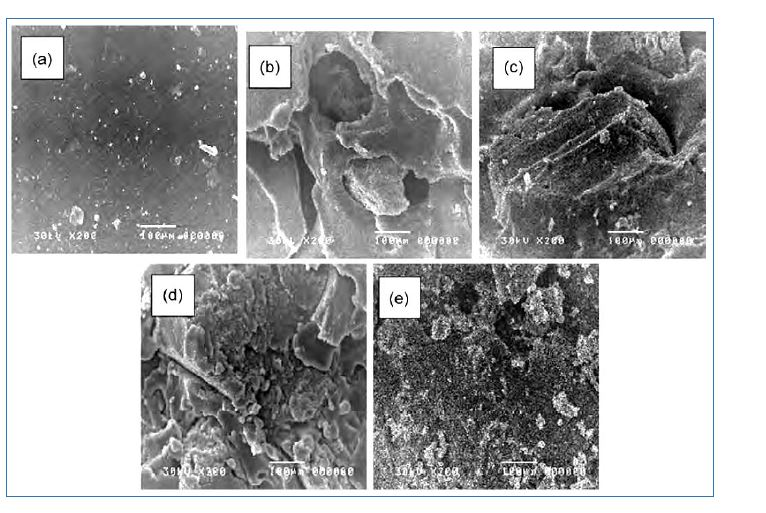
\includegraphics[width=0.9\textwidth]{14.JPG}
			\label{fig:HINH_12}
			\caption{Hình ảnh chụp hiển vi điện tử quét của NBR và hỗn hợp với tỉ lệ trộn khác nhau của RRP: (a) NBR, (b) RRP/NBR/GMA 40/60, (c) RRP/NBR/GMA 50/50, (d) RRP/NBR/GMA 60/40 and RRP}
	\end{figure}	
		
	\begin{figure}
			\centering
			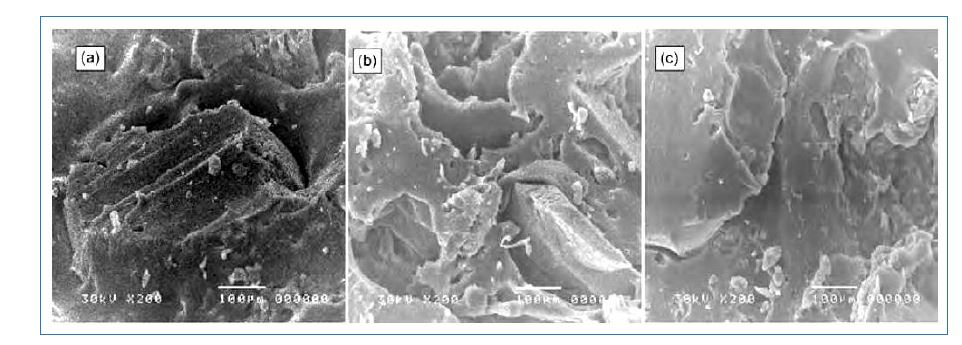
\includegraphics[width=0.9\textwidth]{15.JPG}
			\label{fig:HINH_13}
			\caption{Hình ảnh chụp kính hiển vi điện tử quét của cao su hỗn hợp RRP/NBR/GMA (50/50/2 wt\%) với liều chiếu gamma khác nhau. (a) 0 kGy, (b) 100 kGy , (c) 200 kGy}
	\end{figure}
	
	
	Hình \ref{fig:HINH_12} và \ref{fig:HINH_13} thể hiện kết quả SEM so sánh sự khác biệt về độ đứt gãy bề mặt của cao su hỗn hợp RRP/NBR/GMA không chiếu xạ và chiếu xạ gamma ở độ phóng đại 200. Trong hình chụp SEM của mẫu cao su NBR không chiếu xạ trong hình \ref{fig:HINH_12}(a) cho thấy một vùng có kích thường và hình dạng bất thường của cao su NBR - xuất hiện nhiều trong mạng rỗng xốp. Hình \ref{fig:HINH_12} (c) và (d) thể hiện về mặt hình thái - sự đứt gãy bề mặt khi thay thế một phần NBR với RRP. Hình này thể hiện gần đầy đủ các đặc trưng tương tự ở cùng kích thước và số vùng phân tán của các mẫu. Hình \ref{fig:HINH_12}(b) thể hiện một vùng phân tán thấp và kích thước khít. Điều đó cho thấy rằng trong quá trình tái chế cao su RRP thì sự phá vỡ chuỗi phân tử là diễn ra dữ dội. Hình chụp SEM của mẫu chiếu xạ RRP/NBR/GMA trong hình \ref{fig:HINH_13}(b) và (c) thể hiện vùng bề mặt trơn nhẵn, khi so sánh với \ref{fig:HINH_12}(a) cho thấy rằng các liên kết chéo giữa các thành phần RRP là kết quả của quá trình chiếu xạ gamma. Các hình chụp SEM đã lý giải phần nào độ kéo căng (Tensile strength) giảm khi tăng hàm lượng RRP. Cũng theo hình \ref{fig:HINH_13}(b) về mặt hình dạng của mẫu được chiếu xạ NBR/RRP (50/50) thể hiện tương ứng ở vùng bề mặt trơn nhẵn với nhiều lỗ rỗng và vùng kết tụ không phân tán thì không tìm thấy ở mẫu chiếu xạ
	
	\section{Phần kết luận}
	
	Trong nghiên cứu này nhằm đánh giá mức độ ảnh hưởng khi chiếu xạ gamma lên các tính chất cơ học và lý tính của cao su hỗn hợp tái chế NBR/WRP/GMA. Những kết luận sau được rút ra từ nghiên cứu: .
	
	\begin{enumerate}
	\item[(1)] Độ kéo căng ($T_s$) của mẫu cao su RRP/NBR/GMA không chiếu xạ có giá trị thấp khi thêm RRP. Trong khi đó, giá trị ($T_s$) tăng lên theo liều chiếu tương ứng.
	\item[(2)] Giá trị $E_b$ giảm tuần tự với sự gia tăng hàm lượng RRP được chiếu xạ liều 50kGy. Khi tăng liều chiếu xạ ở toàn bộ mẫu hỗn hợp, thể hiện rằng giá trị $E_b$ tăng lên đến liều 50 kGy rồi sau đó giảm dần.
	\item[(3)] Giá trị độ cứng tăng rõ rệt khi tăng hàm lượng RRP; Ở các mẫu cùng hàm lượng RRP và thành phần thì giá trị độ cứng tăng theo sự gia tăng liều chiếu từ 50 đến 250 kGy.
	\item[(4)] Sự biến thoái do nhiệt giảm dần khi bổ sung thêm cao su phế thải (Waste rubber) vào cao su tái chế hỗn hợp RRP/NBR/GMA và phần trăm khối lượng dư của hỗn hợp tăng rõ rệt khi gia tăng lượng RRP
	\item[(5)] Điều đáng chú ý là phần trăm độ trương phình của cả dầu động cơ và dầu hãm đều giảm khi tăng hàm lượng RRP. Hơn nữa, phần trăm độ trương phình giảm đều khi tăng liều chiếu xạ do sự hình thành các liên kết chéo gây ra bởi bức xạ.
	
	\end{enumerate}
	
	
	
	
	



\end{document}
